\section{Parcelamiento del \'area de Broca}

Estos son los resultados de parcelar el \'area de Broca con un total de 
aproximadamente $760$ semillas. 

\subsection{M\'etodo Moreno-Dominguez}

Las figuras \ref{fig:moreno0} y \ref{fig:moreno1} muestran las parcelas obtenidas 
usando $k=0$ a distintos niveles de profundidad del dendrogama. Las figuras 
\ref{fig:moreno2} y \ref{fig:moreno3} muestran los resultados usando $k=400$ y $k=700$
respectivamente.

\begin{figure}[h!]
    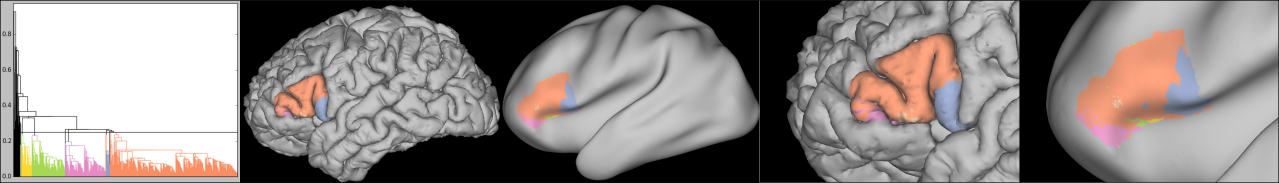
\includegraphics[width=\textwidth]{img/broca/moreno_0.png}
    \caption{M\'etodo Moreno sin restricciones}
    \label{fig:moreno0}
\end{figure}
                                                                                                                       
\begin{figure}[h!]
    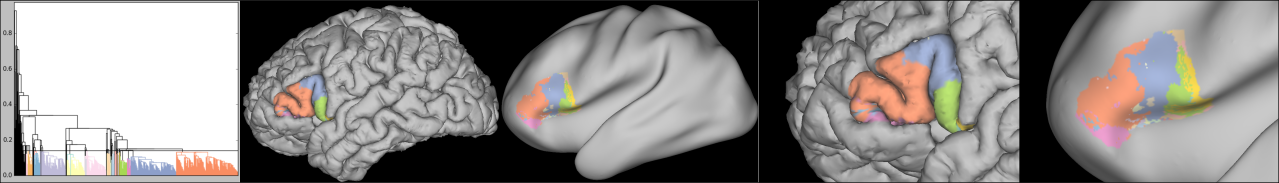
\includegraphics[width=\textwidth]{img/broca/moreno_0_deep.png}
    \caption{M\'etodo Moreno sin restricciones, mayor profundidad en el 
            dendrograma}
    \label{fig:moreno1}
\end{figure}

\begin{figure}[h!]
    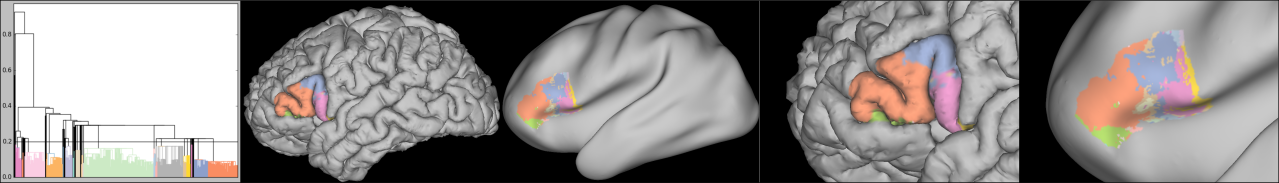
\includegraphics[width=\textwidth]{img/broca/moreno_400.png}
    \caption{M\'etodo Moreno, primeras cuatrocientas uniones entre vecinos}
    \label{fig:moreno2}
\end{figure}

\begin{figure}[h!]
    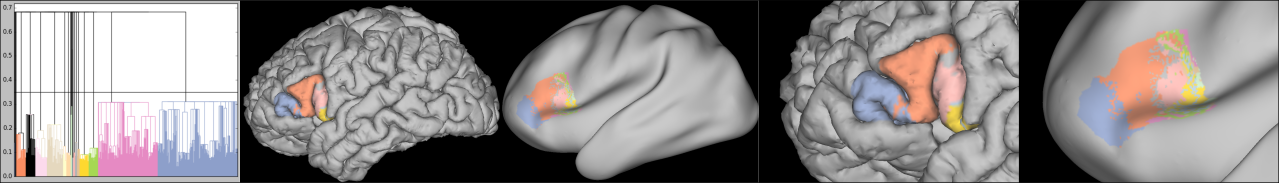
\includegraphics[width=\textwidth]{img/broca/moreno_750.png}
    \caption{M\'etodo Moreno, primeras setecientas uniones entre vecinos}
    \label{fig:moreno3}
\end{figure}

\clearpage

\subsection{Parcelamiento en el espacio eucl\'ideo}

Las figuras \ref{fig:nuestro0} y \ref{fig:nuestro1} muestran las parcelas obtenidas 
usando $k=0$ a distintos niveles de profundidad del dendrogama. Las figuras 
\ref{fig:nuestro2} y \ref{fig:nuestro3} muestran los resultados usando $k=400$ y
$k=700$ respectivamente.

\begin{figure}[h!]
    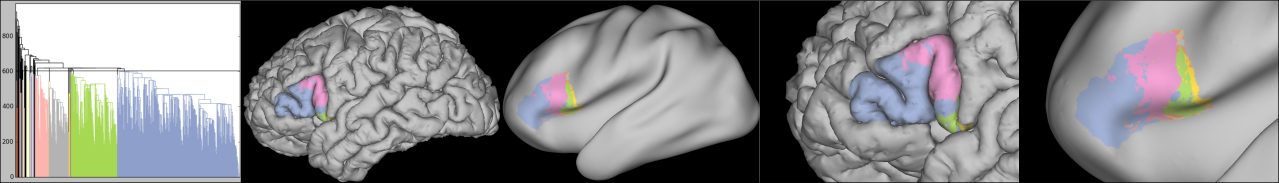
\includegraphics[width=\textwidth]{img/broca/logit_0.png}
    \caption{Nuestro m\'etodo sin restricciones}
    \label{fig:nuestro0}
\end{figure}
                                                                                                                        
\begin{figure}[h!]
    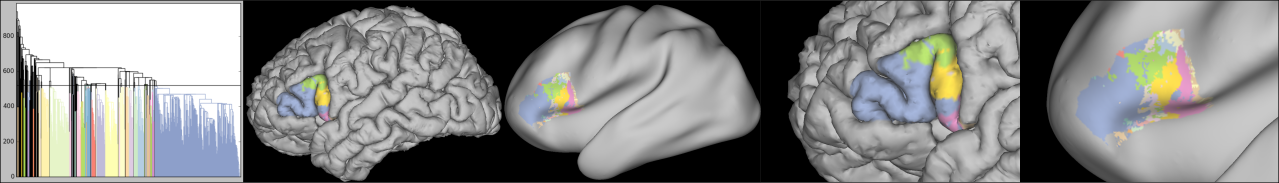
\includegraphics[width=\textwidth]{img/broca/logit_0_deep.png}
    \caption{Nuestro m\'etodo sin restricciones, mayor profundidad en el 
            dendrograma}
    \label{fig:nuestro1}
\end{figure}

\begin{figure}[h!]
    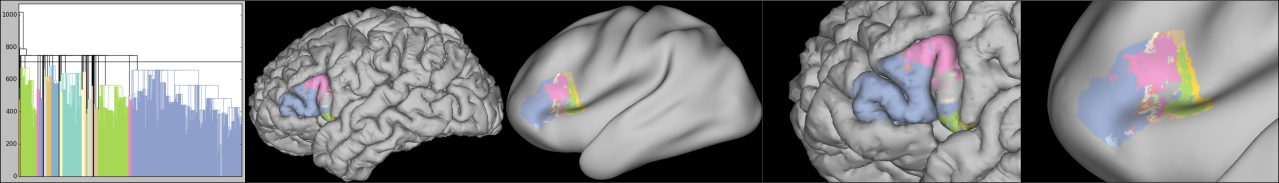
\includegraphics[width=\textwidth]{img/broca/logit_400.png}
    \caption{Nuestro m\'etodo sin preprocesamiento, cuatrocientos pasos de preprocesamiento}
    \label{fig:nuestro2}
\end{figure}

\begin{figure}[h!]
    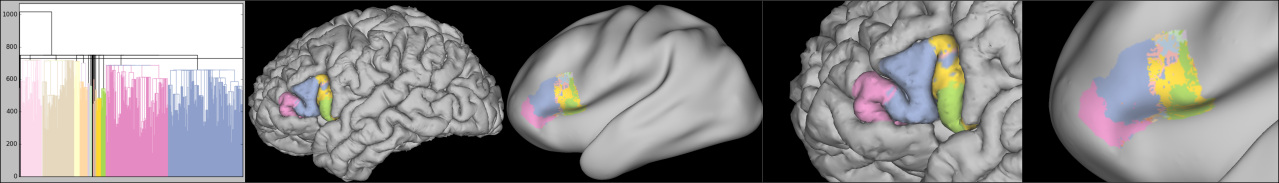
\includegraphics[width=\textwidth]{img/broca/logit_750.png}
    \caption{Nuestro m\'etodo sin preprocesamiento, setecientos pasos de preprocesamiento}
    \label{fig:nuestro3}
\end{figure}

\clearpage

\subsection{Acercamiento a ambos m\'etodos}
\label{sec:acercamiento}

Las figuras \ref{fig:ambos0}; \ref{fig:ambos1} y \ref{fig:ambos2} presentan los
resultados de ambos m\'etodos en simultaneo para $k=0$, $k=400$ y $k=700$ respectivamente.

\begin{figure}[h!]
    \centering
    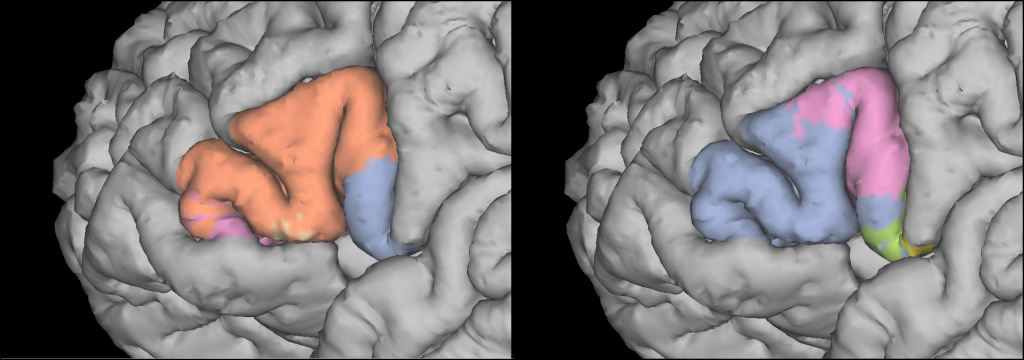
\includegraphics[width=0.9\textwidth]{img/broca/vs_0.png}
    \caption{M\'etodo Moreno-Dominguez (izquierda) y nuestro (derecha) sin preprocesamiento}
    \label{fig:ambos0}
\end{figure}

\begin{figure}[h!]
    \centering
    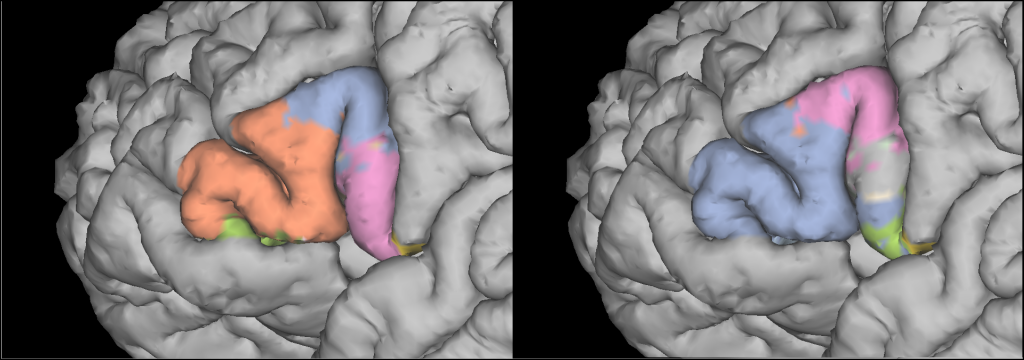
\includegraphics[width=0.9\textwidth]{img/broca/vs_400.png}
    \caption{M\'etodo Moreno-Dominguez (izquierda) y nuestro (derecha). Cuatrocientos pasos de preprocesamiento}
    \label{fig:ambos1}    
\end{figure}
    
\begin{figure}[h!]
    \centering
    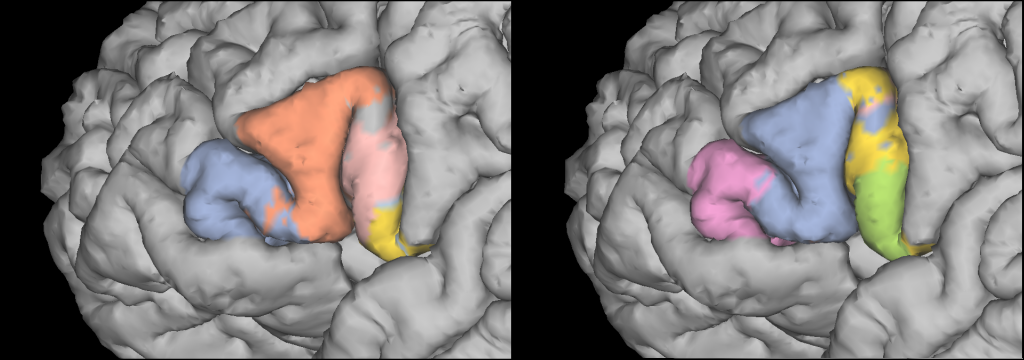
\includegraphics[width=0.9\textwidth]{img/broca/vs_700.png}
    \caption{M\'etodo Moreno-Dominguez (izquierda) y nuestro (derecha). Setecientos pasos de preprocesamiento}
    \label{fig:ambos2}
\end{figure}

\clearpage
